\documentclass[lualatex,handout]{beamer}
\setbeamertemplate{footline}[frame number]
\usepackage{luatexja}
\usepackage{amsmath,amssymb}

%\usetheme{Berlin}
\usecolortheme{rose}

\usepackage{tikz}
\usepackage{pgfplots}
\pgfplotsset{compat=1.18}

%\usepackage[haranoaji]{luatexja-preset}
\usepackage[deluxe,ipaex]{luatexja-preset}
\renewcommand{\kanjifamilydefault}{\gtdefault}
%\setmainjfont{HaranoAjiGothic-Regular}

\usepackage{unicode-math}
%\setmathfont{Fira Math}
\setmathfont{STIX Two Math}
\setmathfont{STIX Two Math}[range=bfup/{Latin,latin,num,Greek,greek}]
\setmathfont{STIX Two Math}[range=bfit/{Latin,latin}]
\setmathfont{STIX Two Math}[range={"0000-"FFFF}]
\setmathrm{STIX Two Math}[StylisticSet=8]

%\usefonttheme{professionalfonts}

\usepackage{luacolor}

\newcommand{\mycolor}[2]{%
  \begingroup
  \colorlet{currentcolor}{.}%
  \color{#1}#2%
  \color{currentcolor}%
  \endgroup
}
\newcommand{\emm}[1]{\mycolor{red}{#1}}
\newcommand{\expt}[1]{\mathbb{E}\left[#1\right]}
\newcommand{\var}[1]{\mathbb{V}\left[#1\right]}
\newcommand{\cov}[1]{\mathsf{Cov}\left[#1\right]}
\newcommand{\vc}[1]{\mathsf{Var}\left[#1\right]}


\usepackage{xspace}
%\usepackage{bm}
%\newcommand\bm[1]{{\mathbf{#1}}}
\newcommand\dx{{\,\mathrm{d}x}}

\theoremstyle{definition}

\title{確率・統計基礎: 複数の確率変数、多変量正規分布}
\author{森 立平}
\date{}



\begin{document}
\begin{frame}[plain]
\maketitle
\end{frame}


\begin{frame}{複数の確率変数の確率密度関数}
\small
\begin{definition}
$p_{Z_1,\dotsc,Z_n}\colon \mathbb{R}\to\mathbb{R}$が
確率変数$Z_1,\dotsc,Z_n$の確率密度関数$\stackrel{\mathrm{def}}{\iff}$
\begin{align*}
\Pr(Z_1\le z_1, Z_2\le z_2,\dotsm Z_n\le z_n)&=
\int_{\substack{-\infty< x_1 \le z_1\\ -\infty< x_2\le z_2\\\vdots\\-\infty<x_n\le z_n}} p_{Z_1,\dotsc,Z_n}(x_1,x_2,\dotsc,x_n)\mathrm{d}{\symbf{x}_1^n}
\end{align*}
\end{definition}
%確率変数$Z_1,\dotsc,Z_n$が\emm{独立}のとき、
%\begin{align*}
%p_{Z_1,\dotsc,Z_n}(x_1,\dotsc,x_n)&=p_{Z_1}(x_1)p_{Z_2}(x_2)\dotsm p_{Z_n}(x_n)
%\end{align*}
%である。
一つの確率変数$Z_1$の確率密度関数は$\Pr(Z_1\le z_1) = \Pr(Z_1\le z_1, Z_2 <\infty,\dotsc, Z_n<\infty)$より
\begin{align*}
p_{Z_1}(x_1)&=
\int_{\substack{-\infty< x_s <\infty \;\forall s\ne 1}} p_{Z_1,\dotsc,Z_n}(x_1,x_2,\dotsc,x_n)\mathrm{d}{\symbf{x}_2^n}.
\end{align*}
他の$Z_k$の確率密度関数についても同様。
\end{frame}

\begin{frame}{独立確率変数}
\begin{align*}
\Pr(Z_1\le z_1, Z_2\le z_2,\dotsm Z_n\le z_n)&=
\Pr(Z_1\le z_1)\Pr(Z_2\le z_2)\dotsm \Pr(Z_n\le z_n)
\end{align*}
\begin{align*}
\int_{\substack{-\infty< x_1 \le z_1\\ -\infty< x_2\le z_2\\\vdots\\-\infty<x_n\le z_n}} p_{Z_1,\dotsc,Z_n}(x_1,x_2,\dotsc,x_n)\mathrm{d}{\symbf{x}_1^n}
&=
\end{align*}
\end{frame}

\begin{frame}{分散共分散行列}
\small
\begin{definition}[分散共分散行列]
確率変数$Z_1,\dotsc,Z_n$の\emm{分散共分散行列}(もしくは\emm{共分散行列})$\vc{\symbf{Z}}\in\mathbb{R}^{n\times n}$は
$(i,\,j)$成分に$\cov{Z_i,\,Z_j}=\expt{Z_iZ_j}-\expt{Z_i}\expt{Z_j}$を持つ行列である。
\end{definition}
\begin{align*}
\vc{\symbf{Z}}&=
\begin{bmatrix}
\var{Z_1}&\cov{Z_1,Z_2}&\cov{Z_1,Z_3}\\
\cov{Z_2,Z_1}&\var{Z_2}&\cov{Z_2,Z_3}\\
\cov{Z_3,Z_1}&\cov{Z_3,Z_2}&\var{Z_3}\\
\end{bmatrix}
\end{align*}
確率変数のベクトルや行列に対する$\expt{\cdot}$は成分毎に期待値を取ることを表す。
\begin{align*}
\symbf{Z} &= \begin{bmatrix}Z_1\\Z_2\\\vdots\\Z_n\end{bmatrix}&\text{とすると}\qquad
\expt{\symbf{Z}} &= \begin{bmatrix}\expt{Z_1}\\\expt{Z_2}\\\vdots\\\expt{Z_n}\end{bmatrix}
\end{align*}
である。
分散共分散行列は以下のように表せる。
\begin{align*}
\symbf{\Sigma}&=
\expt{\symbf{Z} \symbf{Z}^T} - \expt{\symbf{Z}}\expt{\symbf{Z}}^T
\end{align*}
\end{frame}

\begin{frame}{分散共分散行列の性質}
\begin{itemize}
\setlength{\itemsep}{2em}
\item $\vc{\symbf{Z}}$は対称行列である。
\item $\vc{\symbf{Z}}$は半正定値である。
\item $\vc{\symbf{Z}+b}=\vc{\symbf{Z}}\quad\forall b\in\mathbb{R}^n$.
\item $\vc{A\symbf{Z}}=A\vc{\symbf{Z}}A^T\quad\forall A\in\mathbb{R}^{m\times n}$.
%\item $\vc{\symbf{Z}+\symbf{Y}}=\vc{\symbf{Z}} + \vc{\symbf{Y}} + $.
\end{itemize}
\end{frame}

\begin{frame}{線形変換の分散共分散行列}
行列$A\in\mathbb{R}^{m\times n}$と$n\times k$の確率変数行列$\symbf{Z}$について$\expt{A\symbf{Z}}=A\expt{\symbf{Z}}$である。
よって、$N$次元確率変数ベクトル$\symbf{Z}$について
\begin{align*}
&\emm{\expt{(\symbf{Z} - \expt{\symbf{Z}})(\symbf{Z} - \expt{\symbf{Z}})^T}}\\
=&\expt{\symbf{Z}\symbf{Z}^T - \symbf{Z}\expt{\symbf{Z}}^T - \expt{\symbf{Z}}\symbf{Z}^T + \expt{\symbf{Z}}\expt{\symbf{Z}}^T}\\
=& \expt{\symbf{Z} \symbf{Z}^T} - \expt{\symbf{Z}}\expt{\symbf{Z}}^T
=\vc{\symbf{Z}}
\end{align*}
よって$\vc{\symbf{Z}+b}=\vc{\symbf{Z}}$である。

\vspace{1em}
\begin{align*}
\vc{A\symbf{Z}}&=\expt{A\symbf{Z} (A\symbf{Z})^T} - \expt{A\symbf{Z}}\expt{A\symbf{Z}}^T\\
&=A\expt{\symbf{Z} \symbf{Z}^T}A^T - A\expt{\symbf{Z}}\expt{\symbf{Z}}^TA^T\\
&=A\emm{\vc{\symbf{Z}}}A^T
\end{align*}
\end{frame}

\begin{frame}{分散共分散行列の半正定値性 I}
\small
\begin{align*}
&
\begin{bmatrix}
1&\expt{Z_1}&\expt{Z_2}&\expt{Z_3}\\
\expt{Z_1}&\expt{Z_1^2}&\expt{Z_1Z_2}&\expt{Z_1Z_3}\\
\expt{Z_2}&\expt{Z_2Z_1}&\expt{Z_2^2}&\expt{Z_2Z_3}\\
\expt{Z_3}&\expt{Z_3Z_1}&\expt{Z_3Z_2}&\expt{Z_3^2}\\
\end{bmatrix}\\
=&
\expt{
\begin{bmatrix}
1&Z_1&Z_2&Z_3\\
Z_1&Z_1^2&Z_1Z_2&Z_1Z_3\\
Z_2&Z_2Z_1&Z_2^2&Z_2Z_3\\
Z_3&Z_3Z_1&Z_3Z_2&Z_3^2\\
\end{bmatrix}}\\
=&
\expt{
\begin{bmatrix}
1\\
Z_1\\
Z_2\\
Z_3\\
\end{bmatrix}
\begin{bmatrix}
1&
Z_1&
Z_2&
Z_3
\end{bmatrix}}\ge 0\qquad (\text{\emm{半正定値行列の期待値は半正定値}})
\end{align*}

任意の$a\in\mathbb{R}^n$ と$n\times n$半正定値ランダム行列$R$について
$a^T \expt{R}a = \expt{a^TR a}\ge 0$
なので$\expt{R}\ge0$.
\end{frame}

\begin{frame}{分散共分散行列の半正定値性 II}
\scriptsize
\begin{align*}
&
\begin{bmatrix}
-\expt{Z_1}&1&0&0\\
-\expt{Z_2}&0&1&0\\
-\expt{Z_3}&0&0&1\\
\end{bmatrix}
\begin{bmatrix}
1&\expt{Z_1}&\expt{Z_2}&\expt{Z_3}\\
\expt{Z_1}&\expt{Z_1^2}&\expt{Z_1Z_2}&\expt{Z_1Z_3}\\
\expt{Z_2}&\expt{Z_2Z_1}&\expt{Z_2^2}&\expt{Z_2Z_3}\\
\expt{Z_3}&\expt{Z_3Z_1}&\expt{Z_3Z_2}&\expt{Z_3^2}\\
\end{bmatrix}\\
=&
\begin{bmatrix}
0&\expt{Z_1^2}-\expt{Z_1}^2&\expt{Z_1Z_2}-\expt{Z_1}\expt{Z_2}&\expt{Z_1Z_3}-\expt{Z_1}\expt{Z_3}\\
0&\expt{Z_2Z_1}-\expt{Z_2}\expt{Z_1}&\expt{Z_2^2}-\expt{Z_2}^2&\expt{Z_2Z_3}-\expt{Z_2}\expt{Z_3}\\
0&\expt{Z_3Z_1}-\expt{Z_3}\expt{Z_1}&\expt{Z_3Z_2}-\expt{Z_3}\expt{Z_2}&\expt{Z_3^2}-\expt{Z_3}^2\\
\end{bmatrix}\\
\end{align*}
\begin{align*}
&
\begin{bmatrix}
0&\var{Z_1}&\cov{Z_1, Z_2}&\cov{Z_1, Z_3}\\
0&\cov{Z_2, Z_1}&\var{Z_2}&\cov{Z_2, Z_3}\\
0&\cov{Z_3, Z_1}&\cov{Z_3, Z_2}&\var{Z_3}
\end{bmatrix}
\begin{bmatrix}
-\expt{Z_1}& -\expt{Z_2}& -\expt{Z_3}\\
1&0&0\\
0&1&0\\
0&0&1\\
\end{bmatrix}\\
&=\vc{\symbf{Z}}
\end{align*}

$A\ge 0$のとき任意の行列$B$について$BAB^T\ge 0$なので$\vc{\symbf{Z}}\ge 0$である。
\end{frame}

\begin{frame}{多変量正規分布}
\begin{definition}[多変量正規分布]
平均$\mu\in\mathbb{R}^n$、分散共分散行列$\Sigma\in\mathbb{R}^{n\times n}_{>0}$の
多変量正規分布$N(\mu,\,\Sigma)$に従う $n$次元確率変数$\symbf{Z}$の確率密度関数は
\begin{align*}
p_{\symbf{Z}}(x) &= \frac1{\sqrt{(2\pi)^n\det(\Sigma)}} \mathrm{e}^{-\frac12 (x-\symbf{\mu})^T\Sigma^{-1} (x-\symbf{\mu})}
\qquad \text{for }x\in\mathbb{R}^n
\end{align*}
で定義される。

また、$n\times n$単位行列$I_n$について$N(0,\, I_n)$は\emm{$n$次元標準正規分布}と呼ばれる。
\end{definition}
\end{frame}
\begin{frame}{確率密度関数}
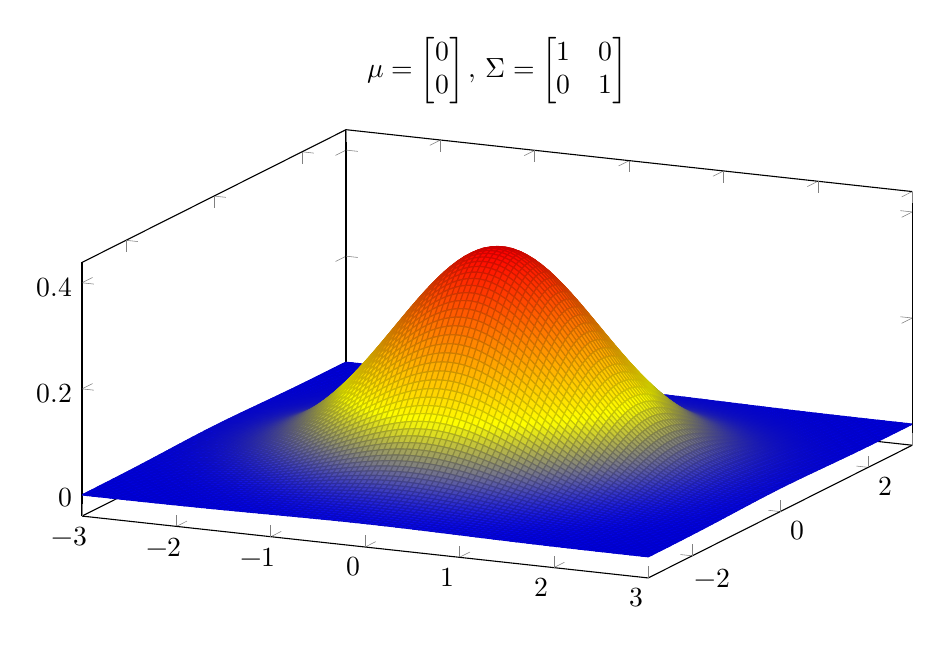
\begin{tikzpicture}
\begin{axis}[
%    title={$\frac1{2\pi}\mathrm{e}^{-\frac12(x^2+y^2)}$},
    title={$\mu=\begin{bmatrix}0\\0\end{bmatrix},\,\Sigma = \begin{bmatrix}1&0\\0&1\end{bmatrix}$},
    width=\textwidth, height=\axisdefaultheight,
%%    zlabel={$p(x,y)$},
%    xlabel={$x$},
%    ylabel={$y$},
%    xmin=-3, xmax=3,
%    ymin=-3, ymax=3,
%    scaled ticks = false,
%    isosamples=100,
%    pm3d = true
    %tick label style={/pgf/number format/assume math mode=true, font=\footnotesize\sffamily},
    %yticklabel style={/pgf/number format/.cd, fixed, fixed zerofill, precision=2},
    %    domain=0:\binomN,samples at={0,1,...,\binomN},
    %mark options={scale=0.75, blue},
    %ybar, bar width = .75pt
        ]
%\addplot[ycomb] {binom(x,\binomN,0.3)};
%\addplot {binom(x,\binomN,0.3)};
\addplot3[surf, domain=-3:3, samples=100] {1.0/sqrt(2*pi) * exp(-0.5*(x^2 + y^2))};
\end{axis}
\end{tikzpicture}
\end{frame}

\begin{frame}{確率密度関数}
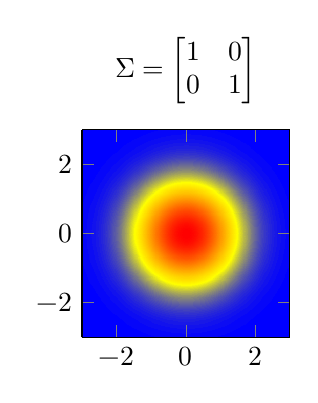
\begin{tikzpicture}
\begin{axis}[
    title={$\Sigma = \begin{bmatrix}1&0\\0&1\end{bmatrix}$},
    width=120, height=120,
    view={0}{90},
    %colorbar horizontal
        ]
\addplot3[contour filled={number=128}, domain=-3:3, samples=100] {1.0/sqrt(2*pi) * exp(-0.5*(x^2 + y^2))};
\end{axis}
\end{tikzpicture}
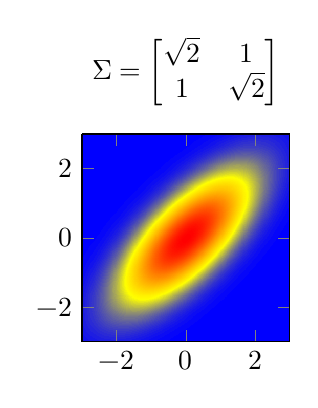
\begin{tikzpicture}
\begin{axis}[
    title={$\Sigma = \begin{bmatrix}\sqrt{2}&1\\1&\sqrt{2}\end{bmatrix}$},
    width=120, height=120,
    view={0}{90},
    %colorbar horizontal
        ]
\addplot3[contour filled={number=128}, domain=-3:3, samples=100] {1.0/sqrt(2*pi) * exp(-0.5*(sqrt(2)*x^2 + sqrt(2)*y^2 - 2*x*y))};
\end{axis}
\end{tikzpicture}
%
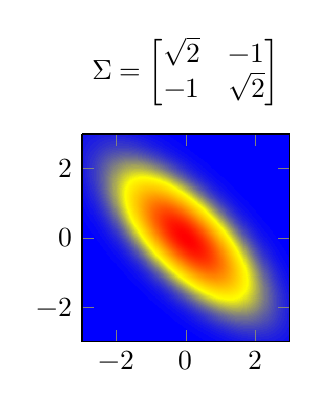
\begin{tikzpicture}
\begin{axis}[
    title={$\Sigma = \begin{bmatrix}\sqrt{2}&-1\\-1&\sqrt{2}\end{bmatrix}$},
    width=120, height=120,
    view={0}{90},
    %colorbar horizontal
        ]
\addplot3[contour filled={number=128}, domain=-3:3, samples=100] {1.0/sqrt(2*pi) * exp(-0.5*(sqrt(2)*x^2 + sqrt(2)*y^2 + 2*x*y))};
\end{axis}
\end{tikzpicture}
\end{frame}

\begin{frame}{密度関数の積分}
\small
多変量正規分布の密度関数を積分して1になることを確認する。
$\Sigma$は対称行列なのである\emm{直交行列$V$}と\emm{対角行列$D$}が存在して$\Sigma=V^TDV$と表せる(スペクトル分解)。
また$\Sigma$は正定値なので、$D$の対角成分は正である。
\begin{align*}
&\int_{\mathbb{R}^n} \frac1{\sqrt{(2\pi)^n\det(\Sigma)}} \mathrm{e}^{-\frac12 (x-\symbf{\mu})^T\Sigma^{-1} (x-\symbf{\mu})}\mathrm{d}x\\
&=
\int_{\mathbb{R}^n} \frac1{\sqrt{(2\pi)^n\det(\Sigma)}} \mathrm{e}^{-\frac12 x^T\Sigma^{-1} x}\mathrm{d}x\\
&=
\int_{\mathbb{R}^n} \frac1{\sqrt{(2\pi)^n\det(D)}} \mathrm{e}^{-\frac12 (Vx)^TD^{-1} (Vx)}\mathrm{d}x\qquad(\Sigma=V^TDV)\\
&=
\int_{\mathbb{R}^n} \frac1{\sqrt{(2\pi)^n\det(D)}} \mathrm{e}^{-\frac12 y^TD^{-1} y}\frac1{|\det(V)|}\mathrm{d}y\qquad (y=Vx)\\
&=
\int_{\mathbb{R}^n} \frac1{\sqrt{(2\pi)^n\det(D)}} \mathrm{e}^{-\frac12 z^T z}\frac1{\left|\det(\sqrt{D^{-1}})\right|}\mathrm{d}z\qquad (z=\sqrt{D^{-1}}y)\\
&=
\int_{\mathbb{R}^n} \frac1{\sqrt{(2\pi)^n}} \mathrm{e}^{-\frac12 z^T z}\mathrm{d}z
=\prod_{k=1}^n\left(\int_{-\infty}^\infty \frac1{\sqrt{2\pi}}\mathrm{e}^{-\frac{z_k^2}2}\mathrm{d}z_k\right) = 1
\end{align*}
\end{frame}

\begin{frame}{多変数のモーメント母関数、キュムラント母関数、特性関数}
\small
\begin{definition}[多変数モーメント母関数]
$n$次元確率変数$X$の\emm{モーメント母関数}$\varphi_{X}\colon\mathbb{R}^n\to\mathbb{R}$を以下で定義する。
\begin{align*}
M_{X}(t) &:= \expt{\mathrm{e}^{\langle t,\, X\rangle}}.
\end{align*}
ここで$\langle t,\, X\rangle := \sum_{k=1}^n t_k X_k$である。

また\emm{キュムラント母関数}を$K_X(t) := \log M_X(t)$と定義する。
\end{definition}
\begin{definition}[多変数特性関数]
$n$次元確率変数$X$の\emm{特性関数}$\varphi_{X}\colon\mathbb{R}^n\to\mathbb{C}$を以下で定義する。
\begin{align*}
\varphi_{X}(t) &:= \expt{\mathrm{e}^{i\langle t,\, X\rangle}}.
\end{align*}
%ここで$\langle t,\, X\rangle := \sum_{k=1}^n t_k X_k$である。
\end{definition}
\end{frame}

\begin{frame}{多変数のモーメント母関数、キュムラント母関数、特性関数の性質}
\small
\begin{itemize}
\setlength{\itemsep}{1em}
\item $M_X(t)$が原点を含む開集合で存在するとき、この範囲で無限回微分でき
\begin{align*}
%\left.\frac{\mathrm{d}^k\varphi_X(t)}{\mathrm{d}t^k}\right|_{t=0} &= i^k \expt{X^k}.
\left.\frac{\partial M_X(t)}{\partial t_k}\right|_{t=0} &= \left.\expt{X_k\mathrm{e}^{\langle t,\, X\rangle}}\right|_{t=0} = \expt{X_k}\\
\left.\frac{\partial^2 M_X(t)}{\partial t_k\partial t_\ell}\right|_{t=0} &= \left.\expt{X_kX_\ell\mathrm{e}^{\langle t,\, X\rangle}}\right|_{t=0} = \expt{X_kX_\ell}\\
\left.\frac{\partial K_X(t)}{\partial t_k}\right|_{t=0} &= \left.\frac{\expt{X_k\mathrm{e}^{\langle t,\, X\rangle}}}{\expt{\mathrm{e}^{\langle t,\, X\rangle}}}\right|_{t=0} = \expt{X_k}\\
\left.\frac{\partial^2 K_X(t)}{\partial t_k\partial t_\ell}\right|_{t=0} &= \left.\frac{\expt{X_kX_\ell\mathrm{e}^{\langle t,\, X\rangle}}}{\expt{\mathrm{e}^{\langle t,\, X\rangle}}}\right|_{t=0} - \left(\left.\frac{\expt{X_k\mathrm{e}^{\langle t,\, X\rangle}}}{\expt{\mathrm{e}^{\langle t,\, X\rangle}}}\right|_{t=0}\right)\left(\left.\frac{\expt{X_\ell\mathrm{e}^{\langle t,\, X\rangle}}}{\expt{\mathrm{e}^{\langle t,\, X\rangle}}}\right|_{t=0}\right)\\
&= \expt{X_kX_\ell} - \expt{X_k}\expt{X_\ell} = \cov{X_k, X_\ell}.
\end{align*}
\item $X$と$Y$の分布が同じ$\emm{\iff}\varphi_X=\varphi_Y$ (ルベーグ積分に基づいた議論が必要).
\end{itemize}


\vspace{1em}
%$X$が$k$次モーメントを持つ$\iff$$\varphi_X$は0で$k$回微分できる。
\end{frame}

\begin{frame}{多変数の特性関数の性質}
\small
\begin{itemize}
\setlength{\itemsep}{3em}
\item $M_{X+b}(t) = \expt{\mathrm{e}^{\langle t,\, X+b\rangle}} = \expt{\mathrm{e}^{\langle t,\, X\rangle}}\mathrm{e}^{\langle t,\,b\rangle}$\\
$\qquad = M_X(t)\mathrm{e}^{\langle t,\, b\rangle}\qquad\forall b\in\mathbb{R}^n$.
\item $M_{AX}(t) = \expt{\mathrm{e}^{\langle t,\, AX\rangle}} = \expt{\mathrm{e}^{\langle A^Tt,\, X\rangle}} = M_X(A^Tt)\qquad\forall A\in\mathbb{R}^{m\times n}$.
\item $M_{X+Y}(t) = \expt{\mathrm{e}^{\langle t,\, X+Y\rangle}} = \expt{\mathrm{e}^{\langle t,\, X\rangle}}\expt{\mathrm{e}^{\langle t,\, Y\rangle}}= M_X(t)M_Y(t)$.
\end{itemize}
\end{frame}

\begin{frame}{多変量正規分布のモーメント母関数}
\small
\begin{align*}
&\expt{\mathrm{e}^{\langle t,\,X\rangle}}\\
&=\int_{-\infty}^\infty \frac1{\sqrt{(2\pi)^n\det(\Sigma)}} \mathrm{e}^{-\frac12 (x-\mu)^T\Sigma^{-1} (x-\mu)}\mathrm{e}^{\langle t,\, x\rangle}\mathrm{d}x\\
&= \int_{-\infty}^\infty \frac1{\sqrt{(2\pi)^n\det(\Sigma)}} \mathrm{e}^{-\frac12 \left\langle\Sigma^{-\frac12}(x-\mu),\,\Sigma^{-\frac12}(x-\mu)\right\rangle+\left\langle \Sigma^{\frac12}t,\, \Sigma^{-\frac12}x\right\rangle}\mathrm{d}x\\
&= \int_{-\infty}^\infty \frac1{\sqrt{(2\pi)^n\det(\Sigma)}} \mathrm{e}^{-\frac12 \left\langle\Sigma^{-\frac12}(x-\mu-\Sigma t),\,\Sigma^{-\frac12}(x-\mu-\Sigma t)\right\rangle +\left\langle \mu,\, t\right\rangle + \frac12\left\langle \Sigma^\frac12t,\,\Sigma^\frac12t\right\rangle}\mathrm{d}x\\
&= \mathrm{e}^{\langle \mu,\, t\rangle + \frac12\langle \Sigma^\frac12t,\,\Sigma^\frac12t\rangle}.
\end{align*}
よって、$K_Z(t) = \emm{\langle \mu,\, t\rangle + \frac12\left\langle \Sigma^\frac12t,\,\Sigma^\frac12t\right\rangle}$.
\begin{align*}
\left.\frac{\partial K_Z(t)}{\partial t_k}\right|_{t=0} &= \mu_k\\
\left.\frac{\partial^2 K_Z(t)}{\partial t_k\partial t_\ell}\right|_{t=0} &= \Sigma_{k, \ell}.
\end{align*}
\end{frame}

\begin{frame}{多変量正規分布$\to$1変数正規分布}
\begin{lemma}
$n$次元の確率変数$\symbf{Z}\sim N(\mu, \Sigma)$について、
$\symbf{Z}':=[Z_1,\dotsc,Z_{n-1}]\sim N(\mu', \Sigma')$.
ここで、$\mu'\in\mathbb{R}^{N-1}$は$\mu$の第$n$成分を除いたもので$\Sigma'$は$\Sigma$の$n$行目と$n$列目を除いたもの。
\end{lemma}
\begin{proof}
\begin{align*}
\varphi_{\symbf{Z}'}(t) &= \expt{\mathrm{e}^{i\langle t,\,Z'\rangle}}\\
&=\expt{\mathrm{e}^{i\langle t,\, Z'\rangle + 0\cdot Z_n}}\\
&=\varphi_{\symbf{Z}}(t,0) = \mathrm{e}^{i\langle t',\,\mu'\rangle - \langle \sqrt{\Sigma'}t,\,\sqrt{\Sigma'}t\rangle}
\end{align*}
\end{proof}
\end{frame}

\begin{frame}{多変量正規分布の一次変換}
\begin{lemma}
$n$次元の確率変数$\symbf{Z}\sim N(\mu, \Sigma)$とランク$m$行列$A\in\mathbb{R}^{m\times n}$と$b\in\mathbb{R}^m$について、
$A\symbf{Z}+b\sim N(A\mu+b, A\Sigma A^T)$.
%$Z_k\sim N(\mu_k, \Sigma_{k,k})$.
\end{lemma}
\begin{proof}
$\varphi_Z(t) = \mathrm{e}^{i\langle \mu,\, t\rangle - \frac12\langle \Sigma^\frac12t,\,\Sigma^\frac12t\rangle}$より、
\begin{align*}
\varphi_{AZ+b}(t) &= \varphi_{AZ}(t)\mathrm{e}^{i\langle t,\,b\rangle} = \varphi_Z(A^Tt)\mathrm{e}^{i\langle t,\,b\rangle}\\
&= \mathrm{e}^{i\langle \mu,\, A^T t\rangle - \frac12\langle \Sigma^\frac12A^T t,\,\Sigma^\frac12A^T t\rangle + i\langle t,\,b\rangle}\\
&= \mathrm{e}^{i\langle A\mu,\, t\rangle - \frac12\langle \Sigma^\frac12A^T t,\,\Sigma^\frac12A^T t\rangle+ i\langle t,\,b\rangle}\\
&= \mathrm{e}^{i\langle A\mu + b,\, t\rangle - \frac12\langle \Sigma^\frac12A^T t,\,\Sigma^\frac12A^T t\rangle}
\end{align*}
これは$N(A\mu+b,\, A\Sigma A^T)$の特性関数である。
\end{proof}
\end{frame}


\begin{frame}{$\chi$二乗分布}
$k$個の独立確率変数が$X_1,\dotsc,X_k\sim N(0,1)$のとき
\begin{align*}
\sum_{s=1}^k X_s^2
\end{align*}
が従う分布を\emm{自由度$k$の$\chi$二乗分布}という。
\end{frame}

%\begin{frame}{標準正規分布に従う確率変数の二乗}
\begin{frame}{自由度1の$\chi$二乗分布}
\small
$f(x)=x^2$は単調関数ではないが$Z$の確率密度関数が対称($p(-z)=p(z)$)のとき、
\begin{align*}
\Pr(Z^2\le x) &= \Pr(Z\in [-\sqrt{x},\,\sqrt{x}])\\
&= \int_{-\sqrt{x}}^{\sqrt{x}} p(z)\mathrm{d}z\\
&= \int_{0}^{\sqrt{x}} p(z)\mathrm{d}z + \int_{-\sqrt{x}}^{0} p(z)\mathrm{d}z\\
&= 2\int_{0}^{\sqrt{x}} p(z)\mathrm{d}z \qquad (p(-z)=p(z))\\
&= 2\int_{0}^{x} p(\sqrt{u})\frac1{2\sqrt{u}}\mathrm{d}u \qquad (u = z^2)
\end{align*}

ここで$Z\sim N(0,1)$のとき、$Z^2$の確率密度関数は以下になる。
\begin{align*}
\emm{\frac1{\sqrt{2\pi x}} \mathrm{e}^{-\frac12 x}}\qquad x \ge 0.
\end{align*}
\end{frame}


\begin{frame}{ガウス積分}
\begin{align*}
&\left(\int_{-\infty}^\infty \frac1{\sqrt{2\pi}}\mathrm{e}^{-\frac12x^2}\mathrm{d}x\right)^2
=
\left(\int_{-\infty}^\infty \frac1{\sqrt{2\pi}}\mathrm{e}^{-\frac12x^2}\mathrm{d}x\right)
\left(\int_{-\infty}^\infty \frac1{\sqrt{2\pi}}\mathrm{e}^{-\frac12y^2}\mathrm{d}y\right)\\
&=
\int_{\mathbb{R}^2} \frac1{2\pi}\mathrm{e}^{-\frac12(x^2+y^2)}\mathrm{d}x\mathrm{d}y\\
&=
\int_{0\le r,\, \theta\in[0,2\pi)} \frac1{2\pi}\mathrm{e}^{-\frac12r^2}r\mathrm{d}r\mathrm{d}\theta\qquad \left(r = \det\left(\begin{bmatrix}\cos\theta&\sin\theta\\-r\sin\theta&r\cos\theta\end{bmatrix}\right)\right)\\
&=
\emm{
\left(\int_{0}^\infty r\mathrm{e}^{-\frac12r^2}\mathrm{d}r\right)
\left(\int_0^{2\pi} \frac1{2\pi}\mathrm{d}\theta\right)}\\
&=\left[-\mathrm{e}^{-\frac12r^2}\right]_0^\infty\cdot 1 = 1
\end{align*}
\end{frame}

\begin{frame}{自由度2の$\chi$二乗分布}
$Z$を自由度2の$\chi$二乗分布に従う確率変数とすると、任意の$A\subseteq\mathbb{R}^2$について
\begin{align*}
\Pr(Z\le z) &= \Pr(X^2 + Y^2 \le z)\\
&= \int_{x^2+y^2\le z} \frac1{2\pi}\mathrm{e}^{-\frac12(x^2+y^2)}\mathrm{d}x\mathrm{d}y\\
&=
\int_{0\le r\le \sqrt{z},\, \theta\in[0,2\pi)} \frac1{2\pi}\mathrm{e}^{-\frac12r^2}r\mathrm{d}r\mathrm{d}\theta\\
&=
\left(\int_{0}^{\sqrt{z}} r\mathrm{e}^{-\frac12r^2}\mathrm{d}r\right)
\left(\int_0^{2\pi} \frac1{2\pi}\mathrm{d}\theta\right)\\
&=\left[-\mathrm{e}^{-\frac12r^2}\right]_0^{\sqrt{z}}\cdot 1 = 1 - \mathrm{e}^{-\frac12 z}
\end{align*}
これを微分すると$\frac12 \mathrm{e}^{-\frac12 z}$である。
これは$U\sim U(0,1)$について\emm{$-2\log U$}の確率密度関数と同じである。
%$Z\sim N(0,1)$のとき、$Z^2$の確率密度関数は以下になる。
%\begin{align*}
%p(x) &= \frac1{\sqrt{2\pi x}} \mathrm{e}^{-\frac12 x}\qquad x \ge 0.
%\end{align*}
%
%\begin{align*}
%&\int_{0}^x p(z)p(x-z)\mathrm{d}z = \int_{0}^x \frac1{2\pi \sqrt{z(x-z)}} \mathrm{e}^{-\frac12 z(x-z)}\mathrm{d}z\\
%&= 2\int_{0}^{\frac{x}2} \frac1{2\pi \sqrt{z(x-z)}} \mathrm{e}^{-\frac12 z(x-z)}\mathrm{d}z\\
%&= 2\int_{0}^{\frac{x^2}4} \frac1{2\pi \sqrt{u}} \mathrm{e}^{-\frac12 u}\frac1{-2z+x}\mathrm{d}u\qquad \left(u=z(x-z),\, z = \frac{x-\sqrt{x^2-4u}}2\right)\\
%&= 2\int_{0}^{\frac{x^2}4} \frac1{2\pi \sqrt{u}} \mathrm{e}^{-\frac12 u}\frac1{\sqrt{x^2-4u}}\mathrm{d}u
%\end{align*}
\end{frame}

\begin{frame}{二次元標準正規分布の極座標表示}
\small
$\begin{bmatrix}X\\ Y\end{bmatrix}\sim N\left(\begin{bmatrix}0\\0\end{bmatrix},\,\begin{bmatrix}1&0\\0&1\end{bmatrix}\right)$について極座標表示$[R, \Theta]$を考える。
つまり、
\begin{align*}
R&:=\sqrt{X^2+Y^2}&\Theta&:=\arctan\frac{Y}{X}\\
X&=R\cos\Theta&Y&=R\sin\Theta
\end{align*}
\begin{align*}
&\Pr([R, \Theta]\in A)\\
&\qquad=
\int_{[r(x,y),\,\theta(x,y)]\in A} \frac1{2\pi}\mathrm{e}^{-\frac12(x^2+y^2)}\mathrm{d}x\mathrm{d}y\\
&\qquad=
\int_{[r,\,\theta]\in A} \frac1{2\pi}\cdot\mathrm{e}^{-\frac12r^2}r\mathrm{d}r\mathrm{d}\theta\\
&\qquad=
\int_{[r,\,\theta]\in A} \emm{p_\Theta(\theta)p_R(r)}\mathrm{d}r\mathrm{d}\theta\\
&\hspace{9em}\left(p_\Theta(\theta):=\frac1{2\pi}\mathbb{1}_{\{\theta\in[0,2\pi)\}},\, p_R(r):=r\mathrm{e}^{-\frac12 r^2}\right).
%\qquad&= \Pr([R\cos\Theta,\, R\sin\Theta]\in A)\qquad (R\sim \chi_2^2, \Theta\sim U(0,2\pi))
\end{align*}
\begin{center}
\large
$R$と$\Theta$は\emm{独立}
\end{center}
%\begin{align*}
%&\Pr([X, Y]\in A)\\
%&\qquad=
%\int_{A} \frac1{2\pi}\mathrm{e}^{-\frac12(x^2+y^2)}\mathrm{d}x\mathrm{d}y\\
%&\qquad=
%\int_{\substack{0\le r,\,\theta\in[0,2\pi)\\ [r\cos\theta,\,r\sin\theta]\in A}} \frac1{2\pi}\cdot\mathrm{e}^{-\frac12r^2}r\mathrm{d}r\mathrm{d}\theta\\
%&\qquad=
%\int_{\substack{0\le r,\,\theta\in[0,2\pi)\\ [r\cos\theta,\,r\sin\theta]\in A}} \emm{p_\Theta(\theta)p_R(r)}\mathrm{d}r\mathrm{d}\theta\\
%&\hspace{9em}\left(p_\Theta(\theta):=\mathbb{1}_{\{\theta\in[0,2\pi)\}},\, p_R(r):=r\mathrm{e}^{-\frac12 r^2}\right)\\
%\qquad&= \Pr([R\cos\Theta,\, R\sin\Theta]\in A)\qquad (R\sim \chi_2^2, \Theta\sim U(0,2\pi))
%\end{align*}
\end{frame}

\begin{frame}{ボックス--ミューラー法}
コンピュータ上でのシミュレーションなどで正規分布に従う乱数はよく用いられる。

\vspace{1em}
コンピュータで標準正規分布に従って実数をランダムに発生させたい。

\vspace{1em}
$U(0,1)$に従ったランダムな実数は発生できると仮定する。

\begin{block}{ボックス--ミューラー法}
\begin{enumerate}
\item $u, v\gets \mathtt{gen\_uniform(0,1)}$.
\item $r \gets \sqrt{-2\log u},\quad \theta \gets 2\pi v$.
\item $x \gets r\cos\theta,\quad y \gets r\sin\theta$.
\end{enumerate}
\emm{この手続きで生成された$x$と$y$は独立な標準正規分布に従う}。
\end{block}

これをくり返すことで独立な標準正規分布に従う乱数をいくらでも作れる。
$X\sim N(0,I)$のとき、$AX + \mu \sim N(\mu, AA^T)$なので一般の多変量正規分布に従う乱数も作れる。
例えば$A=\sqrt{\Sigma}$とすれば$N(\mu,\Sigma)$に従う乱数が発生できる。
\end{frame}

\begin{frame}{直感的な理解と一般化}
二次元標準正規分布の密度関数は\emm{$\sqrt{x^2+y^2}$だけで決まる}。
よって、$\begin{bmatrix}x\\y\end{bmatrix}$を回転しても密度関数の値は不変。
一般に$\begin{bmatrix}X\\Y\end{bmatrix}$の密度関数が$p(x,y)$が$r(x,y)=\sqrt{x^2+y^2}$だけで決まるとき、
$p(x,y)$を$p(r)$と書くことにすると

\begin{align*}
\Pr(R\in A,\,\Theta\in B) &= \int_{r(x,\,y)\in A}\int_{\theta(x,\,y)\in B} p(x,\, y)\mathrm{d}x\mathrm{d}y\\
 &= \int_{r\in A}\int_{\theta\in B} p(r)r\mathrm{d}r\mathrm{d}\theta\\
 &= \left(\int_{\theta\in B}\frac1{2\pi}\mathrm{d}\theta\right)\left(\int_{r\in A} 2\pi rp(r)\mathrm{d}r\right)
\end{align*}

となる。つまり\emm{$R$と$\Theta$は独立で$\Theta$は$[0,2\pi)$上の一様分布}となる。
\end{frame}

\end{document}
